%! TEX root = /home/hsartoris/sproj/writeup/main.tex
\graphicspath{ {resources/models/3neurEx/} {resources/models/3neurEx/weights/} } 

\chapter{Results}
\label{results}
\section{Overfitting}
\label{sec:overfitting}
\setlength{\columnsep}{20pt}
\begin{wraptable}[8]{r}{.4\textwidth}
	\captionsetup{justification=centering}
	\vspace{-20pt}
	\begin{tabular}{lr}
		b (timesteps) & 8\\
		d& 5\\
		Batch size& 32\\
		Training steps& 20000\\
		Learning rate& .0005\\
		Training samples& 18000\\
		Validation samples& 4500
	\end{tabular}
	\vspace{-5pt}
	\captionof{figure}{\linespread{1.2}\selectfont{}Training parameters for null 
		hypothesis networks}
	\label{fig:nullparams}
\end{wraptable}
As discussed in \ref{subsec:hotswap} and \ref{subsec:n-independence}, the unique 
structure of our model prevents it from overfitting to a particular generator 
topology, allowing us to create a single generator containing connections 
representative of the types of data we expect to analyze with the trained model.
We demonstrate this aspect of our architecture in two test cases: by training 
models on an empty dataset paired with one adjacency matrix throughout, and 
training with a random dataset paired with that same adjacency matrix.

\subsection{Empty Data}
\label{subsec:empty}
We ran a combined 100 training sessions of the benchmark model and our 
convolutional model, with parameters as defined in \figref{fig:nullparams}, on a 
dataset whose inputs contained only zeroes and whose target was the adjacency 
matrix in \figref{fig:2simplex+adjacency}. For both models, exactly two losses 
and corresponding outputs repeatedly occurred (\figref{fig:empty_loss}), with 
the models demonstrating a total inability to memorize the target data.

\begin{figure}[h]
	\centering
	\begin{subfigure}{.45\textwidth}
		\centering
		\begin{tabular}{cccc}
				   &  0 &  1 &  2\\\cline{2-4}
			\mc{0} & .3 & .3 & .3\\
			\mc{1} & .3 & .3 & .3\\
			\mc{2} & .3 & .3 & .3
		\end{tabular}
		\caption{loss: $0.\overline{6}$}
		\label{subfig:empty_loss0}
	\end{subfigure}
	\begin{subfigure}{.45\textwidth}
		\centering
		\begin{tabular}{llll}
			  & 0 & 1 & 2\\\cline{2-4}
			\mc{0} & 0 & 0 & 0\\
			\mc{1} & 0 & 0 & 0\\
			\mc{2} & 0 & 0 & 0
		\end{tabular}
		\caption{loss: 1.0}
		\label{subfig:empty_loss1}
	\end{subfigure}
	\caption{Predictions and losses when training on an empty dataset}
	\label{fig:empty_loss}
\end{figure}

\subsection{Random Data}
\label{subsec:random}
\begin{wrapfigure}[7]{r}{.25\textwidth}
	\vspace{-20pt}
	\adjacencyT{0 & .5 & .5}{.5 & 0 & .5}{.5 & .5 & 0}
	\caption{Average prediction for random data. loss: 0.5}
	\label{fig:random_output}
\end{wrapfigure}
For this trial, all model parameters were identical to those in 
\ref{subsec:empty}. In this case, however, the data fed into the network 
consisted of raster plots whose items had been randomly assigned to 0 or 1.  
While the results were somewhat less consistent, over the course of 100 training 
sessions, the models that were able to converge to a minimum loss predicted the 
matrix in \figref{fig:random_output} the overwhelming majority of the time. 

\subsection{Analysis}
While the results of \ref{subsec:random} are at first confusing, given the per 
edge architecture of our model, this result is not particularly surprising: in 
the first layer transition, every spike vector is compared against every other 
spike vector, including itself.  Thus the model was in fact able to learn one 
feature, self loops, and, since loss decreased for driving such connections to 
0, that they do not exist.

For the remainder of the potential connections, the model, lacking any sort of 
way to distinguish between them, found an equilibrium value that, when applied 
to the remaining connectinos, minimized loss. Note that both uniformly 
increasing or decreasing the nonzero weights in \figref{fig:random_output} 
increases loss.

The same is true of the results in \ref{subsec:empty}, with the output in 
\figref{subfig:empty_loss1} particularly illustrative of the problem of entropy 
traps in neural networks. For models that converged to this output, the initial 
seeding of the weight and bias matrices was such that the fastest decreases in 
loss were found by adjusting trainable values to produce an empty matrix. Once 
there, uniformly increasing the output values would initially increase the loss, 
preventing the network from pushing upward and eventually reaching the lower 
loss state of \figref{subfig:empty_loss0}.



\section{3-neuron generator}
\label{results_3neur}
We now consider a generator network consisting of three nodes connected as in 
\figref{fig:2simplex+adjacency}. All weights are binary, and a spike rate of .25 
was used.\footnote{SEE APPENDIX	for information on spike rates} 

\begin{table}[h]
	\centering
	\captionsetup{margin=5em}
	
\begin{tikzpicture}[baseline=(current bounding box.center),->,>=stealth', 
	node distance=5em, semithick]
	\tikzstyle{every state}=[fill=none, draw=black, text=black]

	\node[state] (0) {0};
	\node[state] (1) [right of=0] {1};
	\node[state] (2) [below right of=0] {2};

	\path 	(0) edge node {} (1)
			(0) edge node {} (2)
			(1) edge node {} (2);
\end{tikzpicture}

	\hspace{2em}
	\begin{tabular}{llll}
		& 0 & 1 & 2\\\cline{2-4}
		\mc{0} & 0 & 0 & 0\\
		\mc{1} & 1 & 0 & 0\\
		\mc{2} & 1 & 1 & 0
	\end{tabular}
	\captionof{figure}{Network structure and adjacency matrix of the generator.  
	(Reproduced from Figure \ref{fig:toyex})}
	\label{fig:2simplex+adjacency}
\end{table}\noindent
Reconstructing this simplified graph allows us to demonstrate that our 
convolutional approach is capable of reconstruction.  Furthermore, the small 
generator size requires few timesteps and a small interlayer featurespace; i.e., 
$b,d<10$.  This results in a relatively simple set of transitions, allowing us 
to explore and understand the inner workings of the network.

\subsection{Example Model}
\label{subsec:3neurex}
In order to demonstrate the internal mechanics of our model, we trained on data 
produced by the generator given in \figref{fig:2simplex+adjacency}, with 
parameters as given in \ref{fig:3neur_loss+params}. In this example, small 
values of \textit{b} and \textit{d} were used in order to allow for better 
comprehension and visualization of the internal mechanics; the practical effect 
of this is that relatively small matrices were available for the model to 
optimize, making each value adjustment more impactful on output, and thus each 
training step more dramatic.  These are acceptable limitations, however, insofar 
as they provide a more comprehensible model struture.

\begin{table}[ht]
	\centering
	\begin{minipage}{.48\textwidth}
	\resizebox{\textwidth}{!}{
		\begin{tikzpicture}
			\begin{semilogyaxis} [xlabel=Step, ylabel=Loss, scaled x 
				ticks=false,
				axis lines*=left,
				xtick={1,3750,7500,11250,15000},
				extra y ticks={.05,.5}, extra y tick style={grid=major},
%				ytick={0,.1,.5,1}, 
				yticklabel style={	/pgf/number format/precision=2,
									/pgf/number format/fixed}]
				\addplot [color=black] table [x=Step, y=Loss, col sep=comma, 
			mark=none, smooth] {../resources/models/3neurEx/losses};
			\end{semilogyaxis}
		\end{tikzpicture}
	}
	\end{minipage}
	\hfill
	\begin{minipage}{.48\textwidth}
		\centering
		\begin{tabular}{lr}
			b (timesteps) & 8\\
			d& 5\\
			Batch size& 32\\
			Learning rate& .0005\\
			Training samples& 17984\\
			Validation samples& 4512
		\end{tabular}
	\end{minipage}
	\captionof{figure}{Training loss and parameters for model described in 
	\ref{subsec:3neurex}. The loss here is somewhat choppier than usual, due to 
the limited matrix size made available to the model.}
	\label{fig:3neur_loss+params}
\end{table}


\subsection{Trained Network Operation}
Here, we will consider a single item of data as it travels through the model 
trained in \ref{subsec:3neurex}.

\label{subsec:trainedoperation}
\begin{figure}[h]
	\centering
	\begin{subfigure}{.15\textwidth}
		\centering
		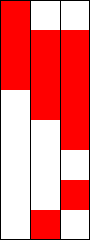
\includegraphics[width=.75\textwidth]{fullRun/0_py/input.png}
		\caption{Input\\(max: 1.0)}
		\label{subfig:3neur_in}
	\end{subfigure}
	\hspace{.5em}
	\begin{subfigure}{.35\textwidth}
		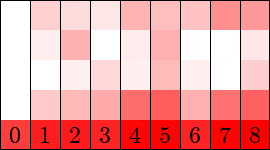
\includegraphics[width=\textwidth]{fullRun/0_py_num/layer0/4out.png}
		\caption{Output of first layer\\(max: 4.33)}
	\end{subfigure}
	\hspace{1em}
	\begin{subfigure}{.35\textwidth}
		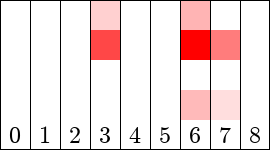
\includegraphics[width=\textwidth]{fullRun/0_py_num/layer1/7out.png}
		\caption{Output of second layer\\(max: 3.2)}
		\label{subfig:3neur_out1}
	\end{subfigure}
	\\
	\begin{subfigure}{.35\textwidth}
		\centering
		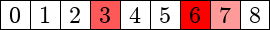
\includegraphics[width=\textwidth]{fullRun/0_py_num/layerf/0out.png}
		\caption{Output of final layer\\(max: 30.97)}
		\label{subfig:3neur_outf}
	\end{subfigure}
	\begin{subfigure}{.3\textwidth}
		\centering
		
\includegraphics[width=.5\textwidth]{fullRun/0_py/pred.png}
		\caption{Prediction\\(max: 1.0)}
		\label{subfig:3neur_pred}
	\end{subfigure}
	\caption{Path of data through network. Transparency for each value is scaled 
	relative to the maximum value found in the matrix.}
	\label{fig:3neur_run}
\end{figure}\noindent
In \figref{fig:3neur_run}, we demonstrate the progression of 
\ref{subfig:3neur_in} through the trained model. The final layer, including 
activation\footnote{See \ref{subsec:finalactivation}}, produces an $n^2$-vector 
which, when reshaped into an $(n \times n)$ matrix, is an exact match for the 
target, with all connections located and weighted appropriately.\footnote{While 
	$[1,0]$ and $[2,0]$ are predicted to be exactly 1.0, the precise value of 
	$[2,1]$ in the final prediction is 0.999999999957586, which we consider to 
be accurate enough.}
%The final layer turns the information from \ref{subfig:3neur_out1} into a 
%prediction by multiplying the matrix found in \ref{subfig:3neur_flayer} with 
%\ref{subfig:3neur_out1} to produce \ref{subfig:3neur_outf}, which is then 
%passed into the final layer activation function\footnote{See 
%\ref{subsec:finalactivation}} and reshaped to $(n \times n)$ to produce 
%\ref{subfig:3neur_pred}, an exact match for the target with all connections 
%located and weighted appropriately.\footnote{While $[1,0]$ and $[2,0]$ are 
%predicted to be exactly 1.0, the precise value of $[2,1]$ in the final 
%prediction is 0.999999999957586, which we consider to be accurate enough.}
\subsubsection{Analysis}
blah blah blah it's all well and good that this works

\paragraph{First Layer Functionality}

\paragraph{Convolutional Layer Functionality}

Note that, following the convolutional layer (\ref{subfig:3neur_out1}), the 
model has located the existent connections: if we transpose 
\ref{subfig:3neur_out1} from $(d \times n^2)$ to $(n \times n \times d)$, as in 
\figref{fig:transform}, the columns with high values, 3, 6, and 7, correspond 
with \textit{d}-vectors $[1,0]$, $[2,0]$, and $[2,1]$, respectively. These 
tuples each correspond with a connection present in the adjacency matrix 
(\figref{fig:toyex}) the model is trying to predict. 

\paragraph{Final Layer}
\begin{wrapfigure}[5]{r}{.25\textwidth}
	\centering
	\vspace{-15pt}
	
\includegraphics[width=.25\textwidth]{fullRun/0_py/layerf/weights.png}
	\caption{Final weights\\(max: 7.31)}
	\label{fig:3neur_flayer}
\end{wrapfigure}
The final layer consists only of multiplying its weights 
(\figref{fig:3neur_flayer}) by the output from the previous layer, and it is 
thus relatively easy to intepret what the model has learned at this stage. As 
the first two values of of the weight matrix are strongly positive, we can 
conlude that the first two values in each vector in the output from the previous 
layer are highly important in the determination of connection presence, with 
some weight also placed on the fourth item.

\section{Higher-order Datasets}
Because a 3-node generator does contain much in terms of locality, we created 
and generated data from the following generator:
\begin{table}[h]

\begin{tikzpicture}[baseline=(current bounding box.center),->,>=stealth', 
	node distance=5em, semithick]
	\tikzstyle{every state}=[fill=none, draw=black, text=black]

	\node[state] (0) {0};
	\node[state] (1) [right of=0] {1};
	\node[state] (2) [below left of=1] {2};
	\node[state] (3) [right of=1] {3};
	\node[state] (4) [right of=3] {4};
	\node[state] (5) [below left of=4] {5};
	\node[state] (6) [right of=5] {6};
	\node[state] (7) [above right of=6] {7};
	\node[state] (8) [right of=6] {8};
	\node[state] (9) [below left of=3] {9};

	\path 	(0) edge node {} (1)
			(0) edge node {} (2)
			(1) edge node {} (2)
			(4) edge node {} (5)
			(6) edge node {} (7)
			(7) edge node {} (8);
\end{tikzpicture}

	

\end{table}


\section{Applicability Beyond Training Data}
As described in \ref{subsec:hotswap}, the fact that our model is trained on data 
produced by only one generator is of little consequence; due to its structure, 
the only information it can learn is relational; i.e., per-neuron-pair. Consider 
the following examples, in which data was produced from several generator 
networks and fed into the model described in \ref{results_3neur}:


TODO: add examples of input and output data to 3.2.1 and 3.2.2.

\subsection{Inverted Network}
\begin{table}[h]
	\centering
	\begin{tikzpicture}[baseline=(current bounding box.center),->,>=stealth', 
	node distance=5em, semithick]
	\tikzstyle{every state}=[fill=none, draw=black, text=black]

		\node[state] (0) {0};
		\node[state] (1) [right of=0] {1};
		\node[state] (2) [below right of=0] {2};
	
		\path 	(2) edge node {} (1)
				(2) edge node {} (0)
				(1) edge node {} (0);
	\end{tikzpicture}
	\hspace{2em}
	\begin{tabular}{l|lll}
		  & 0 & 1 & 2\\
		\hline
		0 & 0 & 1 & 1\\
		1 & 0 & 0 & 1\\
		2 & 0 & 0 & 0
	\end{tabular}
	\captionof{figure}{Inverted version of \figref{fig:2simplex+adjacency}}
	\label{fig:2simplexVar1}
\end{table}
\noindent Despite being a complete inversion of the generator used to train the 
model in \ref{results_3neur}, reconstruction of this network is simple.

\begin{table}[h]
	\centering
	\begin{minipage}{.1\textwidth}
		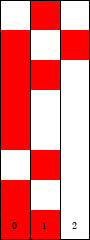
\includegraphics[width=\textwidth]{var1/input.png}
	\end{minipage}
	\hspace{2em}
	{\scalebox{2}{$\Rightarrow$}}
	\hspace{2em}
	\begin{tabular}{l|lll}
		  & 0 & 1 & 2\\
		\hline
		0 & .01 & 1.00 & 1.00\\
		1 & .01 & .02 & 1.00\\
		2 & 0 & .02 & .01
	\end{tabular}
\end{table}

\subsection{Cyclical Network}
\label{subsec:cyclical}
\begin{table}[h]
	\centering
	\begin{tikzpicture}[baseline=(current bounding box.center),->,>=stealth', 
	node distance=5em, semithick]
	\tikzstyle{every state}=[fill=none, draw=black, text=black]

		\node[state] (0) {0};
		\node[state] (1) [right of=0] {1};
		\node[state] (2) [below right of=0] {2};
	
		\path 	(2) edge node {} (1)
				(0) edge node {} (2)
				(1) edge node {} (0);
	\end{tikzpicture}
	\hspace{2em}
	\begin{tabular}{l|lll}
		  & 0 & 1 & 2\\
		\hline
		0 & 0 & 1 & 0\\
		1 & 0 & 0 & 1\\
		2 & 1 & 0 & 0
	\end{tabular}
	\captionof{figure}{Cyclical 3-neuron network}
	\label{fig:2simplexVar2}
\end{table}

\noindent For a cyclical network, the situation is not quite so simple. Due to 
the perpetual propagation of spikes through the generator, additional random 
spiking can cause the input data to become an impenetrable mess. Tempering the 
spike rate to 0.05 produces workable data, but the results are neither so clean 
nor
consistent as for terminating networks.  


